\documentclass[a4paper]{article}

% Introduction block (usepackages,settings,...)
\usepackage{amsmath} % Define various maths environments
\usepackage{amsthm}
\usepackage{amssymb} % Define various maths symbols
\usepackage{geometry} % Adjust the margin, paper size, and etc.
\usepackage{enumerate} % Provide different style of lists
\usepackage{graphicx} % Insert image of all types
\usepackage{xcolor}
\usepackage{ulem}
\usepackage{pdfpages}
\usepackage{array} % Provide auxiliary farmat for tabular
\usepackage{booktabs} % Create Three-line Table
\usepackage{bm}
\usepackage{cite}
\usepackage{url}
\usepackage{float}
\usepackage{indentfirst}
\usepackage{multirow}
\usepackage{verbatim}
% Use other packages and setup them here


\begin{document}

\vspace*{0.4cm}

\hrulefill %??????draw a horizontal line??????

\thispagestyle{empty} %set empty in footnote

\begin{center}
\begin{large}
\scshape{UM--SJTU Joint Institute \vspace{0.3em} \\ Physics Laboratory \\(Vp141)}
\end{large}

\hrulefill %??????draw a horizontal line??????

\vspace*{6cm}
\begin{Large}
\scshape{{Laboratory Report}}
\end{Large}

\vspace{2em}

\begin{large}
\scshape{Exercise 5}\\
\vspace{0.5em}
\scshape{Damped and Driven Oscillations.}\\
\scshape{Mechanical Resonance}\\
\end{large}
\end{center}
\vfill %??????

\begin{table}[htbp] %what function does "h!" perform?
\flushleft
\begin{tabular}{lll}
Name: Kang Jiaming \hspace*{3em} & ID: 518021911220 \hspace*{3em} & Group: 18\\
Name: Luo Chenhao \hspace*{3em} & ID: 518370910038 \hspace*{3em} & Group: 18\\
\\
\end{tabular}
\end{table}

\hfill %??????
\newpage
\tableofcontents
\setcounter{page}{0} %set the next page (the first page of the body) as page 1
\thispagestyle{empty}
\newpage



\section{Introduction}\label{Sec:intro}

The objective of this exercise is to further the knowledge about damped and driven mechanical oscillations, and also the mechanical resonance phenomenon. How to operate on the Pohl resonator will also be explored.

For a simple harmonic oscillator, its equation of motion is $\displaystyle\frac{d^{2} x}{d t^{2}}+ \frac{k}{m}x = 0.$ If the oscillator experiences a linear drag, its motion becomes a damped harmonic oscillation, and the equation of motion is $\displaystyle\frac{d^{2} x}{d t^{2}}+ b \frac{d x}{d t} + \frac{k}{m}x = 0.$ If further, a driving force is applied to the damped harmonic oscillator, the resulting motion is called driven (or forced) oscillations. Assuming that the driving force is of the form $\displaystyle F=F_{0} \cos \omega t,$ the equation of motion is then:
\begin{equation}\label{Eq:linearequation}
\frac{d^{2} x}{d t^{2}}+ b \frac{d x}{d t} + \frac{k}{m}x = F_{0} \cos \omega t.
\end{equation}
It can be observed that the driven oscillation will be a periodic motion with the same angular frequency $\omega$ after it stabilizes.

In this experiment, however, the oscillation system takes the angular form instead of linear form. A balance wheel, the oscillator in our system, rotates about its central axis, with the restoring torque $\displaystyle\tau=-k \theta$, a damping torque $\displaystyle\tau_{f}=-b \frac{d \theta}{d t}$ and a periodic driving torque $\displaystyle\tau_{\mathrm{dr}}=\tau_{0} \cos \omega t$. Its equation of motion is then
\begin{equation}\label{Eq:angularoriginequation}
I \frac{d^{2} \theta}{d t^{2}}=-k \theta-b \frac{d \theta}{d t}+\tau_{0} \cos \omega t.
\end{equation}
Simplifying the notions using$\displaystyle\omega_{0}^{2}=\frac{k}{I}, \quad 2 \beta=\frac{b}{I}, \quad \mu=\frac{\tau_{0}}{I}$, Eq.\ref{Eq:angularoriginequation} can be written as
\begin{equation}\label{Eq:angularequation}
\frac{d^{2} \theta}{d t^{2}}+2 \beta \frac{d \theta}{d t}+\omega_{0}^{2} \theta=\mu \cos \omega t.
\end{equation}

The solution to Eq.\ref{Eq:angularequation} is
\begin{equation}\label{Eq:angularsolution}
\theta(t)=\theta_{\mathrm{tr}}(t)+\theta_{\mathrm{st}} \cos (\omega t+\varphi).
\end{equation}
$\theta_{\mathrm{tr}}$ represents the influence of initial conditions on the motion, which vanishes exponentially as $t \rightarrow \infty$. $\theta_{\mathrm{st}} \cos (\omega t+\varphi)$ describes the motion of the steady states. Its amplitude $\theta_{\mathrm{st}}$ and the phase shift $\varphi$ are found as
\begin{equation}\label{Eq:amplitude}
\theta_{\mathrm{st}}=\frac{\mu}{\sqrt{\left(\omega_{0}^{2}-\omega^{2}\right)^{2}+4 \beta^{2} \omega^{2}},}
\end{equation}
and
\begin{equation}\label{Eq:phaselag}
\tan \varphi=\frac{2 \beta \omega}{\omega^{2}-\omega_{0}^{2}} \: (-\pi \leq \varphi<0),
\end{equation}
The figures of $\theta_{\mathrm{st}}$ vs. $\omega$ (left) and $\varphi$ vs. $\omega$ (right)are shown in Figure \ref{Fig:graph}.

From Eq.\ref{Eq:amplitude}, it can be derived that when $\omega$ becomes closed to $\omega_{0}$, the amplitude will sharply increase. Such a phenomenon is called resonance. It can also be obtained that when $\omega = \omega_{res} = \sqrt{\omega_{0}^{2}-2 \beta^{2}}$, which is called the resonance angular frequency, the amplitude reaches its maximum
\begin{equation}\label{Eq:resonanceamplitude}
\theta_{\mathrm{res}}=\theta_{\mathrm{st}}\left(\omega_{\mathrm{res}}\right)=\frac{\mu}{2 \beta \sqrt{\omega_{0}^{2}-\beta^{2}}}
\end{equation}

\begin{figure}[htpb]
\begin{center}
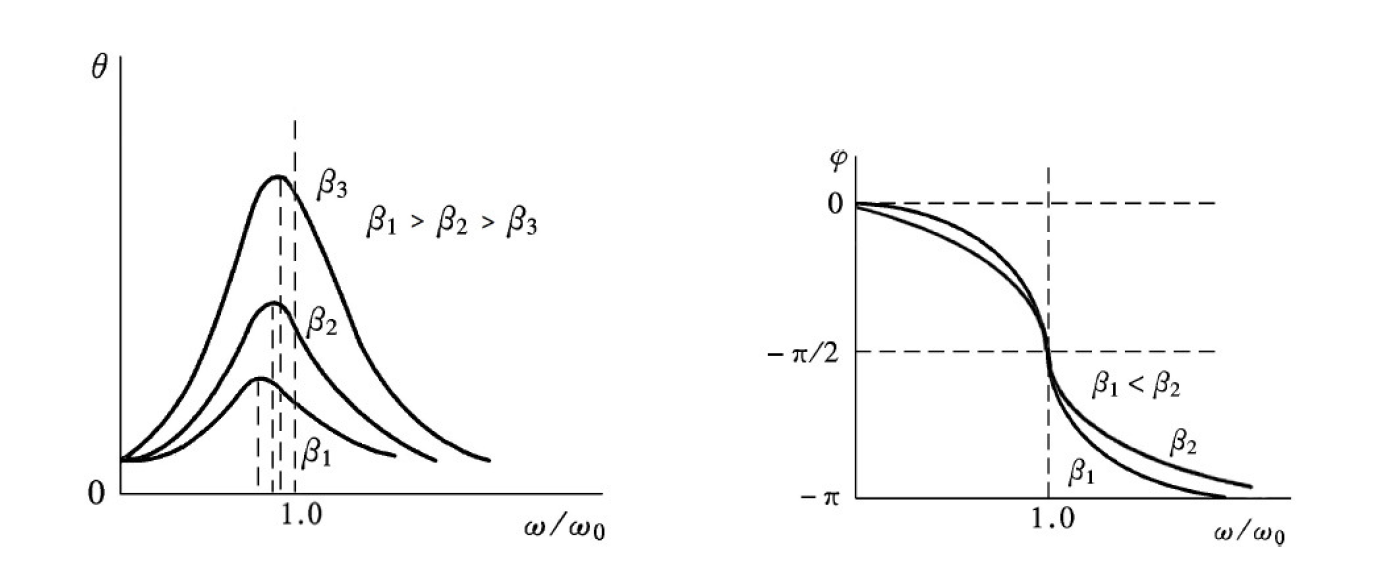
\includegraphics[width=0.8\textwidth]{graph.png}
\caption{The dependence of the amplitude (left) and phase shift (right) of steady-state driven oscillations.}\label{Fig:graph}
\end{center}
\end{figure}

As for the basic ideas for measurement, period $T$ and angular frequency $\omega$ are related by the formula
\begin{equation}\label{Eq:omega}
\omega = \frac{2 \pi}{T}.
\end{equation}
Therefore, the angular frequency can be found by measuring the period of oscillations.
The solution to Eq.\ref{Eq:angularequation} combining the initial state and the final steady state is $\theta(t)=\theta e^{-\beta t} \cos \left(\omega_{\mathrm{f}} t+\alpha\right)$. Hence, if we measure the amplitude every other period and obtain $\theta_{0}=\theta e^{-\beta T}, \theta_{1}=\theta e^{-\beta(2 T)},\ldots$ $, \theta_{n}=\theta e^{-\beta(n T)}$, we have
\begin{equation}\label{Eq:predampingrelation}
\ln \frac{\theta_{i}}{\theta_{j}}=\ln \frac{\theta e^{-\beta(i T)}}{\theta e^{-\beta(j T)}}=(j-i) \beta T
\end{equation}
The damping coefficient $\beta$ can be then calculated as
\begin{equation}\label{Eq:predampingcoefficient}
\beta=\frac{1}{(j-i) T} \ln \frac{\theta_{i}}{\theta_{j}}
\end{equation}

In our experiment, we will measure ten items of data, i.e. $\theta_{0},\theta_{1},\ldots,\theta_{9}$. But how should we process the measurement data? Shall we simply takes $j=i+1$, achieve ten $\beta$, and calculate the average as the result?

In that case, the average value is expressed by
\begin{equation}
\beta = \frac{\frac{1}{T} \ln \frac{\theta_{0}}{\theta_{1}} + \frac{1}{T} \ln \frac{\theta_{1}}{\theta_{2}} + \cdots + \frac{1}{T} \ln \frac{\theta_{8}}{\theta_{9}}}{10} = \frac{\ln \frac{\theta_{0}}{\theta_{9}}}{10T}
\end{equation}
It can be seen that actually only $\theta_{0}$ and $\theta_{9}$ are taken into account. How to deal with the data so that all the data can be used?

The successive difference method is an effective method to reduce the error of the average value calculated from a series of measurement data. Applying the idea to our experiment, we take $j=i+5$ and the damping coefficient is thus calculated as
\begin{equation}\label{Eq:damping}
\beta=\frac{1}{5 T} \ln \frac{\theta_{i}}{\theta_{i+5}}
\end{equation}
In this case, the average value is expressed by
\begin{equation}\label{Eq:dampingaverage}
\beta = \frac{\frac{1}{T} \ln \frac{\theta_{0}}{\theta_{5}} + \frac{1}{T} \ln \frac{\theta_{1}}{\theta_{6}} + \cdots + \frac{1}{T} \ln \frac{\theta_{4}}{\theta_{9}}}{5} = \frac{\ln \frac{\theta_{0}\theta_{1}\cdots\theta_{4}}{\theta_{5}\theta_{6}\cdots\theta_{9}}}{5T}
\end{equation}
In Eq.\ref{Eq:dampingaverage}, all the data measured is used. The error can be reduced in this way.

\section{Experimental Setup} \label{Sec:exset}

The whole experimental is conducted through a BG-2 Pohl resonator which consists of a vibrometer (Figure \ref{Fig:vibrometer}) and a control box (Figure \ref{Fig:controlboxfront} and \ref{Fig:controlboxrear}). Period can be measured by the timer in the control box. Phase lag can be read off from the angle scale on the balance wheel which a flash generated by the strobe shines onto. Amplitude can also be displayed by the control box. The knobs on the control box can change the magnitude of the damping force and the frequency of the driving force.

\begin{figure}[htbp]
\begin{center}
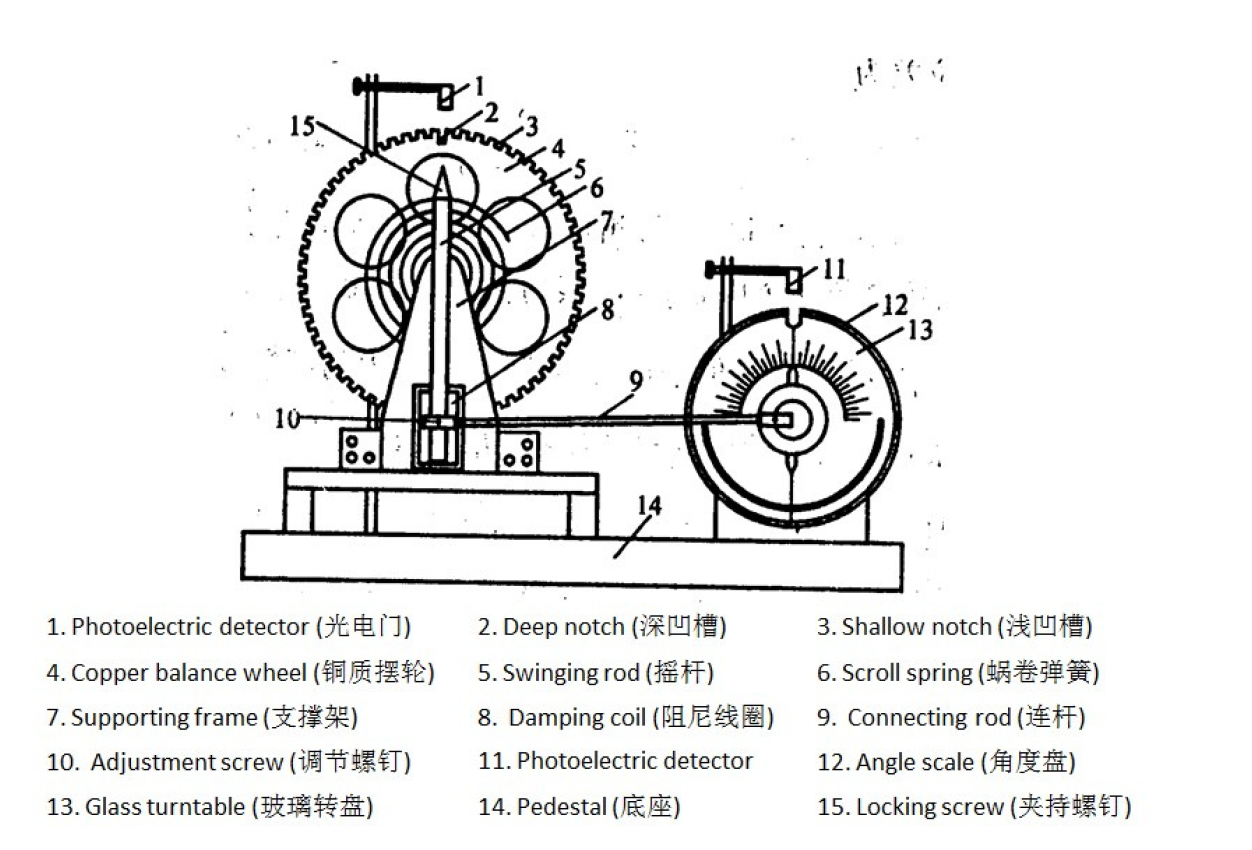
\includegraphics[width=0.8\textwidth]{vibrometer.png}
\caption{The vibrometer.}\label{Fig:vibrometer}
\end{center}
\end{figure}

\begin{figure}[htbp]
\begin{center}
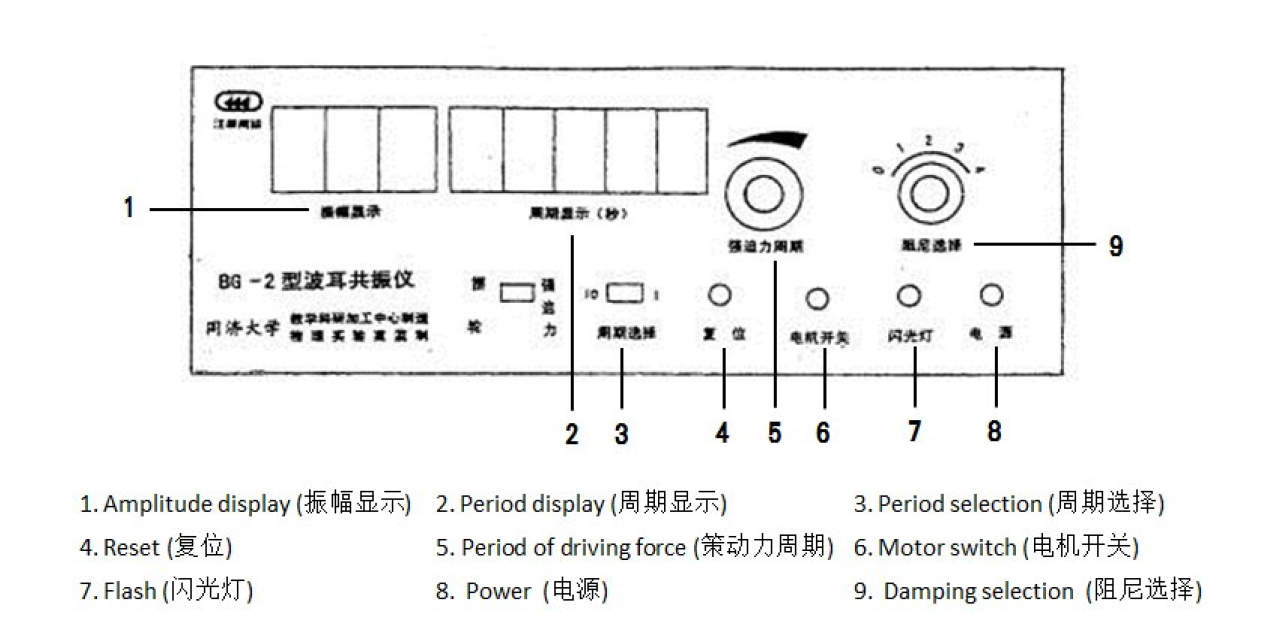
\includegraphics[width=0.8\textwidth]{controlboxfront.png}
\caption{The front panel of the control box.}\label{Fig:controlboxfront}
\end{center}
\end{figure}

\begin{figure}[htbp]
\begin{center}
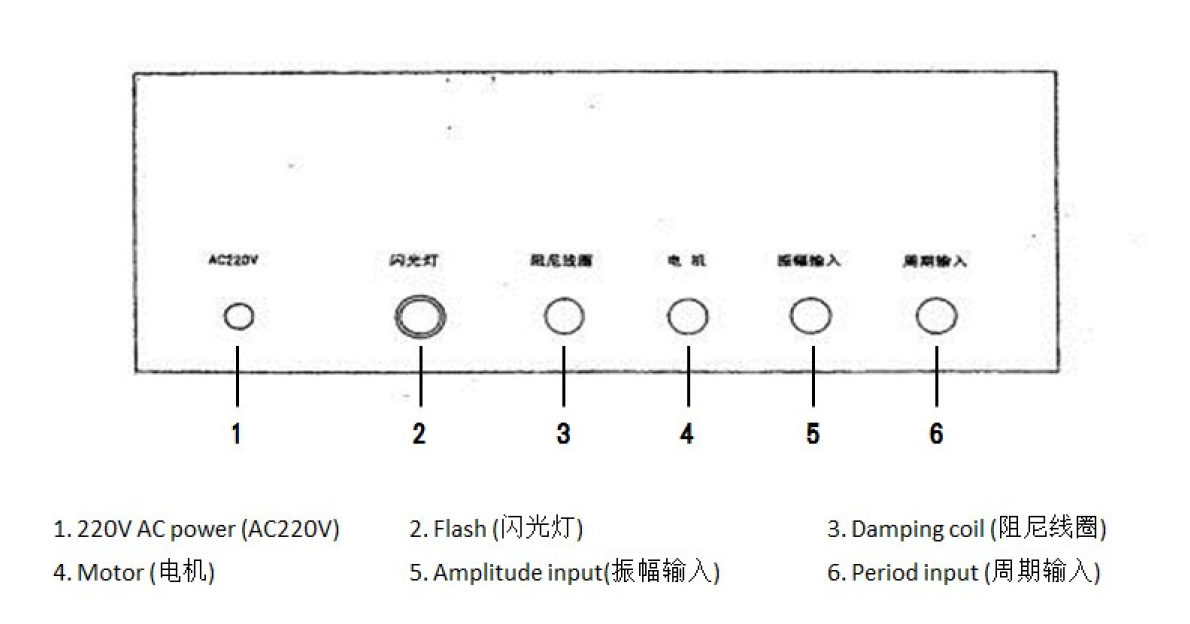
\includegraphics[width=0.8\textwidth]{controlboxrear.png}
\caption{The rear panel of the control box.}\label{Fig:controlboxrear}
\end{center}
\end{figure}

The type-B uncertainties of the measured physical quantities are summarized in Table \ref{Tab:typebuncertainties}.

\begin{table}[htbp]
\begin{center}
\begin{tabular}{cc}
\hline
Physical quantities & Type-B uncertainties \\ \hline
Ten periods         & 0.001\,s             \\
Amplitude           & 1\,$^{\circ}$        \\
Phase lag           & 1\,$^{\circ}$        \\ \hline
\end{tabular}
\caption{Type-B uncertainties.}\label{Tab:typebuncertainties}
\end{center}
\end{table}



\section{Measurement Procedure}\label{Sec:mepro}

\subsection*{CAUTION}
\begin{enumerate}
\item Check the position of the photoelectric gate above the balanced wheel. Make sure there is enough space between the gate and the wheel.
\item Pohl resonator is a very delicate device, you should operate the apparatus according to the manual and instructions of the teaching assistant.
\item The motor must be turned off during steps \ref{mepronatural} and \ref{meprodamping}.
\item To ensure accuracy of the measurement, you should not change the $\textsf{Damping Selection}$ until the entire measurement is completed.
\end{enumerate}

\subsection{Natural Angular Frequency}\label{mepronatural}
The natural angular frequency is obtained by simply measuring the period of the oscillation without damping and driving force and applying Eq.\ref{Eq:omega}.
\begin{enumerate}
\item Turn the $\textsf{Damping Selection}$ knob to "0". 
\item Carefully rotate the balance wheel to the initial angular position $\theta_0 \approx 150^\circ$ and release it. Record the time of 10 periods.
\item Repeat for four times and calculate the natural angular frequency $\omega_0$.
\end{enumerate}

\subsection{Damping Coefficient}\label{meprodamping}
The damping coefficient is found by measuring the amplitude every other period and applying Eq.
Note that the first measured amplitude should be neglected since the oscillation at first may be affected by the operators.
\ref{Eq:damping}.
\begin{enumerate}
\item Turn the $\textsf{Damping Selection}$ knob to "2", and the selection should not be changed during this part.
\item Carefully rotate the balance wheel to the initial amplitude of approximately $150^\circ$ and release it. Record the amplitude of each period (start from the second amplitude after you release the wheel) and the time of 10 periods. \\
$\textit{Tip.}$ In case you miss some readings, repeat the measurement recording it with your phone camera.
\item Apply Eq.\ref{Eq:damping} and calculate the average of the results to find $\beta$
\end{enumerate}

\subsection{$\theta_{st}$ vs. $\omega$ and $\varphi$ vs. $\omega$ Characteristics of Forced Oscillations}\label{proc3}
In this part, driving force will be applied to the oscillation system. Its frequency should be adjusted in a well-designed way as instructed in step 2 in order to get sufficient data to plot the $\theta_{st}$ vs. $\omega$ and $\varphi$ vs. $\omega$ graphs.

Please be patient enough to wait for the oscillation stabilizes. It is recommended to wait for at least ten seconds after the amplitude stays unchanged.

When measuring the phase lag, the flash will not occur exactly at the same position. Read a medium scale in that case.
\begin{enumerate}
\item Keep the $\textsf{Damping Selection}$ at "2", and set the speed of the motor (record the position of the motor knob in case you need to repeat the measurement). Record the amplitude $\theta_{st}$, the period $T$, and the phase shift $\varphi$ when the oscillation reaches a steady state.
\item Repeat the steps above by changing the speed of the motor. It will result in a change of the phase shift $\varphi$ (referred to as $\delta\varphi$). To make your plots more accurate, you should collect more data when $\varphi$ and $\theta_{st}$ change rapidly ($e.g.$ near to the resonance point). At least 15 data should be collected for plotting.
\item Choose $\textsf{Damping Selection}$ "1" or "3". Repeat the above steps.
\item Plot the $\theta_{st}(\omega)$ characteristics, with $\omega/\omega_0$ on the horizontal axis and $\theta_{st}$ on the vertical axis. Two sets of data should be plotted on the same graph.
\\Plot the $\varphi(\omega)$ characteristics, with $\omega/\omega_0$ on the horizontal axis and $\varphi$ on the vertical axis. Two sets of data should be plotted on the same graph.

\end{enumerate}



\section{Results}

\subsection{Natural Angular Frequency}

The measured time of 10 periods is presented in Table \ref{Tab:naturalfrequency}

\begin{table}[htbp]
\centering
\begin{tabular}{cc}
\toprule
Trial & $T_{10}\,[\text{s}] \pm 0.001\,[\text{s}]$ \\
\midrule
1 & 15.881\\
2 & 15.881\\
3 & 15.879\\
4 & 15.879\\
\bottomrule
\end{tabular}
\caption{Measurement results of the natural frequency.}\label{Tab:naturalfrequency}
\end{table}

The average value of $T_{10}$ is 
\[\overline{T_{10}} = \frac{1}{4} \sum \limits_{i=1}^{4} T_{10_{i}} = 15.880 \pm 0.00208\,[\text{s}].\]

The average value of T is thus
\[\overline{T} = \frac{1}{10} \overline{T_{10}} = 1.5880 \pm 0.0002\,[\text{s}].\]

Hence, applying Eq.\ref{Eq:omega}, the natural frequency is 
\[\omega_{0} = \frac{2\pi}{\overline{T}} = \frac{2\pi}{1.5880} = 3.9567 \pm 0.0005\,[\text{s}^{-1}],\]
with relative uncertainty 0.01\,\%


\subsection{Damping Coefficient}

The time of ten periods measured is $T_{10} = 15.892 \pm 0.001 \,\text{s}.$

The measured data of amplitude is presented in Table \ref{Tab:damping}
\begin{table}[htbp]
\centering
\begin{tabular}{cc|cc|c}
\toprule
Item & Amplitude$[^\circ]\pm 1[^\circ]$ &Item & Amplitude$[^\circ]\pm 1[^\circ]$ & $q_i=\text{ln}(\theta_i/\theta_{i+5})$\\
\midrule
$\theta_0$ & 128 & $\theta_5$ & 78 & 0.495 $\pm$ 0.015\\
$\theta_1$ & 116 & $\theta_6$ & 70 & 0.505 $\pm$ 0.017\\
$\theta_2$ & 104 & $\theta_7$ & 62 & 0.517 $\pm$ 0.019\\
$\theta_3$ & 95 & $\theta_8$ & 56 & 0.529 $\pm$ 0.021\\
$\theta_4$ & 87 & $\theta_9$ & 51 & 0.534 $\pm$ 0.023\\
\bottomrule
\end{tabular}
\caption{Measurement results of the damping coefficient.}\label{Tab:damping}
\end{table}

From Table \ref{Tab:damping} we can calculate
\[\overline{q} = \frac{1}{5} \sum \limits_{i=1}^{5} q_i = 0.516 \pm 0.030.\]

The period $T$ is
\[T = \frac{1}{10}\times 15.892 = 1.5892 \pm 0.0001\,[\text{s}].\]

Thus, we can calculate the damping coefficient $\beta$ by applying Eq.\ref{Eq:damping}:
\[\beta=\frac{1}{5 T} \overline{q} = 0.064938 \pm 0.004\,[\text{s}^{-1}],\]
with relative uncertainty 6.16\,\%


\subsection{$\theta$ vs. $\omega$ and $\varphi$ vs. $\omega$ Characteristics of Forced Oscillations}
In the first trial, the $\textsf{Damping Selection}$ is ``2'' and the data is presented in Table \ref{Tab:pregraphdamping2}; in the second trial, the $\textsf{Damping Selection}$ is ``1'' and the data is presented in Table \ref{Tab:pregraphdamping1} 

\begin{table}[htbp]
\centering
\begin{tabular}{cccc}
\toprule
Trial & $T_{10}\,[\text{s}]\pm0.001\,[\text{s}]$ & $\varphi\,[^\circ]\pm1\,[^\circ]$ & $\theta\,[^\circ]\pm 1\,[^\circ]$\\
\midrule
1 &16.613&	20&	48\\
2 &16.408&	27&	63\\
3 &16.274&	34&	80\\
4 &16.152&	44&	99\\
5 &16.095&	51&	110\\
6 &16.023&	62&	123\\
7 &15.962&	73&	133\\
8 &15.925&	81&	138\\
9 &15.906&	85&	138\\
10 &15.893&	88&	138\\
11 &15.886&	89&	138\\
12 &18.879&	91&	138\\
13 &15.864&	95&	138\\
14 &15.855&	97&	138\\
15 &15.848&	99&	137\\
16 &15.843&	100&	136\\
17 &15.783&	113&	127\\
18 &15.719&	126&	112\\
19 &15.655&	135&	98\\
20 &15.592&	142&	85\\
21 &15.524&	147&	73\\
22 &15.407&	154&	58\\
23 &15.255&	159&46\\
24 &15.045&	163&	35\\
\bottomrule
\end{tabular}
\caption{Measurement results when $\textsf{Damping Selection}$ is``2''.\label{Tab:pregraphdamping2}}
\end{table}

\begin{table}[htbp]
\centering
\begin{tabular}{cccc}
\toprule
Trial & $T_{10}\,[\text{s}]\pm0.001\,[\text{s}]$ & $\varphi\,[^\circ]\pm1\,[^\circ]$ & $\theta\,[^\circ]\pm 1\,[^\circ]$\\
\midrule
1&16.575	&20	&51\\
2&16.411	&25	&64\\
3&16.227	&36	&89\\
4&16.139	&44	&104\\
5&16.072	&53	&118\\
6&16.015	&62	&131\\
7&15.964	&72	&140\\
8&15.918	&82	&146\\
9&15.901	&86	&148\\
10&15.893	&88	&148\\
11&15.887	&89	&148\\
12&15.878	&91	&148\\
13&15.865	&94	&148\\
14&15.843	&100	&146\\
15&15.786	&114	&136\\
16&15.709	&130	&114\\
17&15.603	&143	&89\\
18&15.448	&154	&64\\
19&15.269	&161	&47\\
20&15.077	&164	&36\\
\bottomrule
\end{tabular}
\caption{Measurement results when $\textsf{Damping Selection}$ is ``1''.\label{Tab:pregraphdamping1}}
\end{table}



Calculate $T_{10_\text{natural}}/T_{10}$, which is equal to $\omega/\omega_0$, and the corresponding uncertainties. The results are shown in Table \ref{Tab:graphdamping2} and \ref{Tab:graphdamping1}.

\begin{table}[htbp]
\centering
\begin{tabular}{cccccc}
\toprule
Trial & $T_{10}\,[\text{s}]\pm0.001\,[\text{s}]$ & $\varphi\,[^\circ]\pm1\,[^\circ]$ & $\theta\,[^\circ]\pm 1\,[^\circ]$ & $\omega/\omega_0$ & $u_{\omega/\omega_0}$\\
\midrule
1&16.613	&20	&48	&0.9559 	&0.0001 \\
2&16.408	&27	&63	&0.9678 	&0.0001 \\
3&16.274	&34	&80	&0.9758 	&0.0001 \\
4&16.152	&44	&99	&0.9832 	&0.0001 \\
5&16.095	&51	&110	&0.9866 	&0.0001 \\
6&16.023	&62	&123	&0.9911 	&0.0001 \\
7&15.962	&73	&133	&0.9949 	&0.0001 \\
8&15.925	&81	&138	&0.9972 	&0.0001 \\
9&15.906	&85	&138	&0.9984 	&0.0001 \\
10&15.893	&88	&138	&0.9992 	&0.0001 \\
11&15.886	&89	&138	&0.9996 	&0.0001 \\
12&18.879	&91	&138	&0.8411 	&0.0001 \\
13&15.864	&95	&138	&1.0010 	&0.0001 \\
14&15.855	&97	&138	&1.0016 	&0.0001 \\
15&15.848	&99	&137	&1.0020 	&0.0001 \\
16&15.843	&100	&136	&1.0023 	&0.0001 \\
17&15.783	&113	&127	&1.0061 	&0.0001 \\
18&15.719	&126	&112	&1.0102 	&0.0001 \\
19&15.655	&135	&98	&1.0144 	&0.0001 \\
20&15.592	&142	&85	&1.0185 	&0.0001 \\
21&15.524	&147	&73	&1.0229 	&0.0001 \\
22&15.407	&154	&58	&1.0307 	&0.0002 \\
23&15.255	&159	&46	&1.0410 	&0.0002 \\
24&15.045	&163	&35	&1.0555 	&0.0002 \\
\bottomrule
\end{tabular}
\caption{$\omega/\omega_0$ and corresponding uncertainties when $\textsf{Damping Selection}$ is "2".}\label{Tab:graphdamping2}
\end{table}



\begin{table}[htbp]
\centering
\begin{tabular}{cccccc}
\toprule
Trial & $T_{10}\,[\text{s}]\pm0.001\,[\text{s}]$ & $\varphi\,[^\circ]\pm1\,[^\circ]$ & $\theta\,[^\circ]\pm 1\,[^\circ]$ & $\omega/\omega_0$ & $u_{\omega/\omega_0}$\\
\midrule
1&16.575	&20	&51	&0.9581 	&0.0001 \\
2&16.411	&25	&64	&0.9676 	&0.0001 \\
3&16.227	&36	&89	&0.9786 	&0.0001 \\
4&16.139	&44	&104	&0.9840 	&0.0001 \\
5&16.072	&53	&118	&0.9881 	&0.0001 \\
6&16.015	&62	&131	&0.9916 	&0.0001 \\
7&15.964	&72	&140	&0.9947 	&0.0001 \\
8&15.918	&82	&146	&0.9976 	&0.0001 \\
9&15.901	&86	&148	&0.9987 	&0.0001 \\
10&15.893	&88	&148	&0.9992 	&0.0001 \\
11&15.887	&89	&148	&0.9996 	&0.0001 \\
12&15.878	&91	&148	&1.0001 	&0.0001 \\
13&15.865	&94	&148	&1.0009 	&0.0001 \\
14&15.843	&100	&146	&1.0023 	&0.0001 \\
15&15.786	&114	&136	&1.0060 	&0.0001 \\
16&15.709	&130	&114	&1.0109 	&0.0001 \\
17&15.603	&143	&89	&1.0178 	&0.0001 \\
18&15.448	&154	&64	&1.0280 	&0.0002 \\
19&15.269	&161	&47	&1.0400 	&0.0002 \\
20&15.077	&164	&36	&1.0533 	&0.0002 \\
\bottomrule
\end{tabular}
\caption{$\omega/\omega_0$ and corresponding uncertainties when $\textsf{Damping Selection}$ is "1".\label{Tab:graphdamping1}}
\end{table}



With the data in Table \ref{Tab:pregraphdamping2} $\sim$ \ref{Tab:graphdamping1}, plot $\theta_{st}$ vs. $\omega/\omega_0$ and $\varphi$ vs. $\omega/\omega_0$ using Origin. The results are presented in Figure \ref{Fig:amplitude} and Figure \ref{Fig:phaselag} respectively.

\begin{figure}[htbp]
\centering
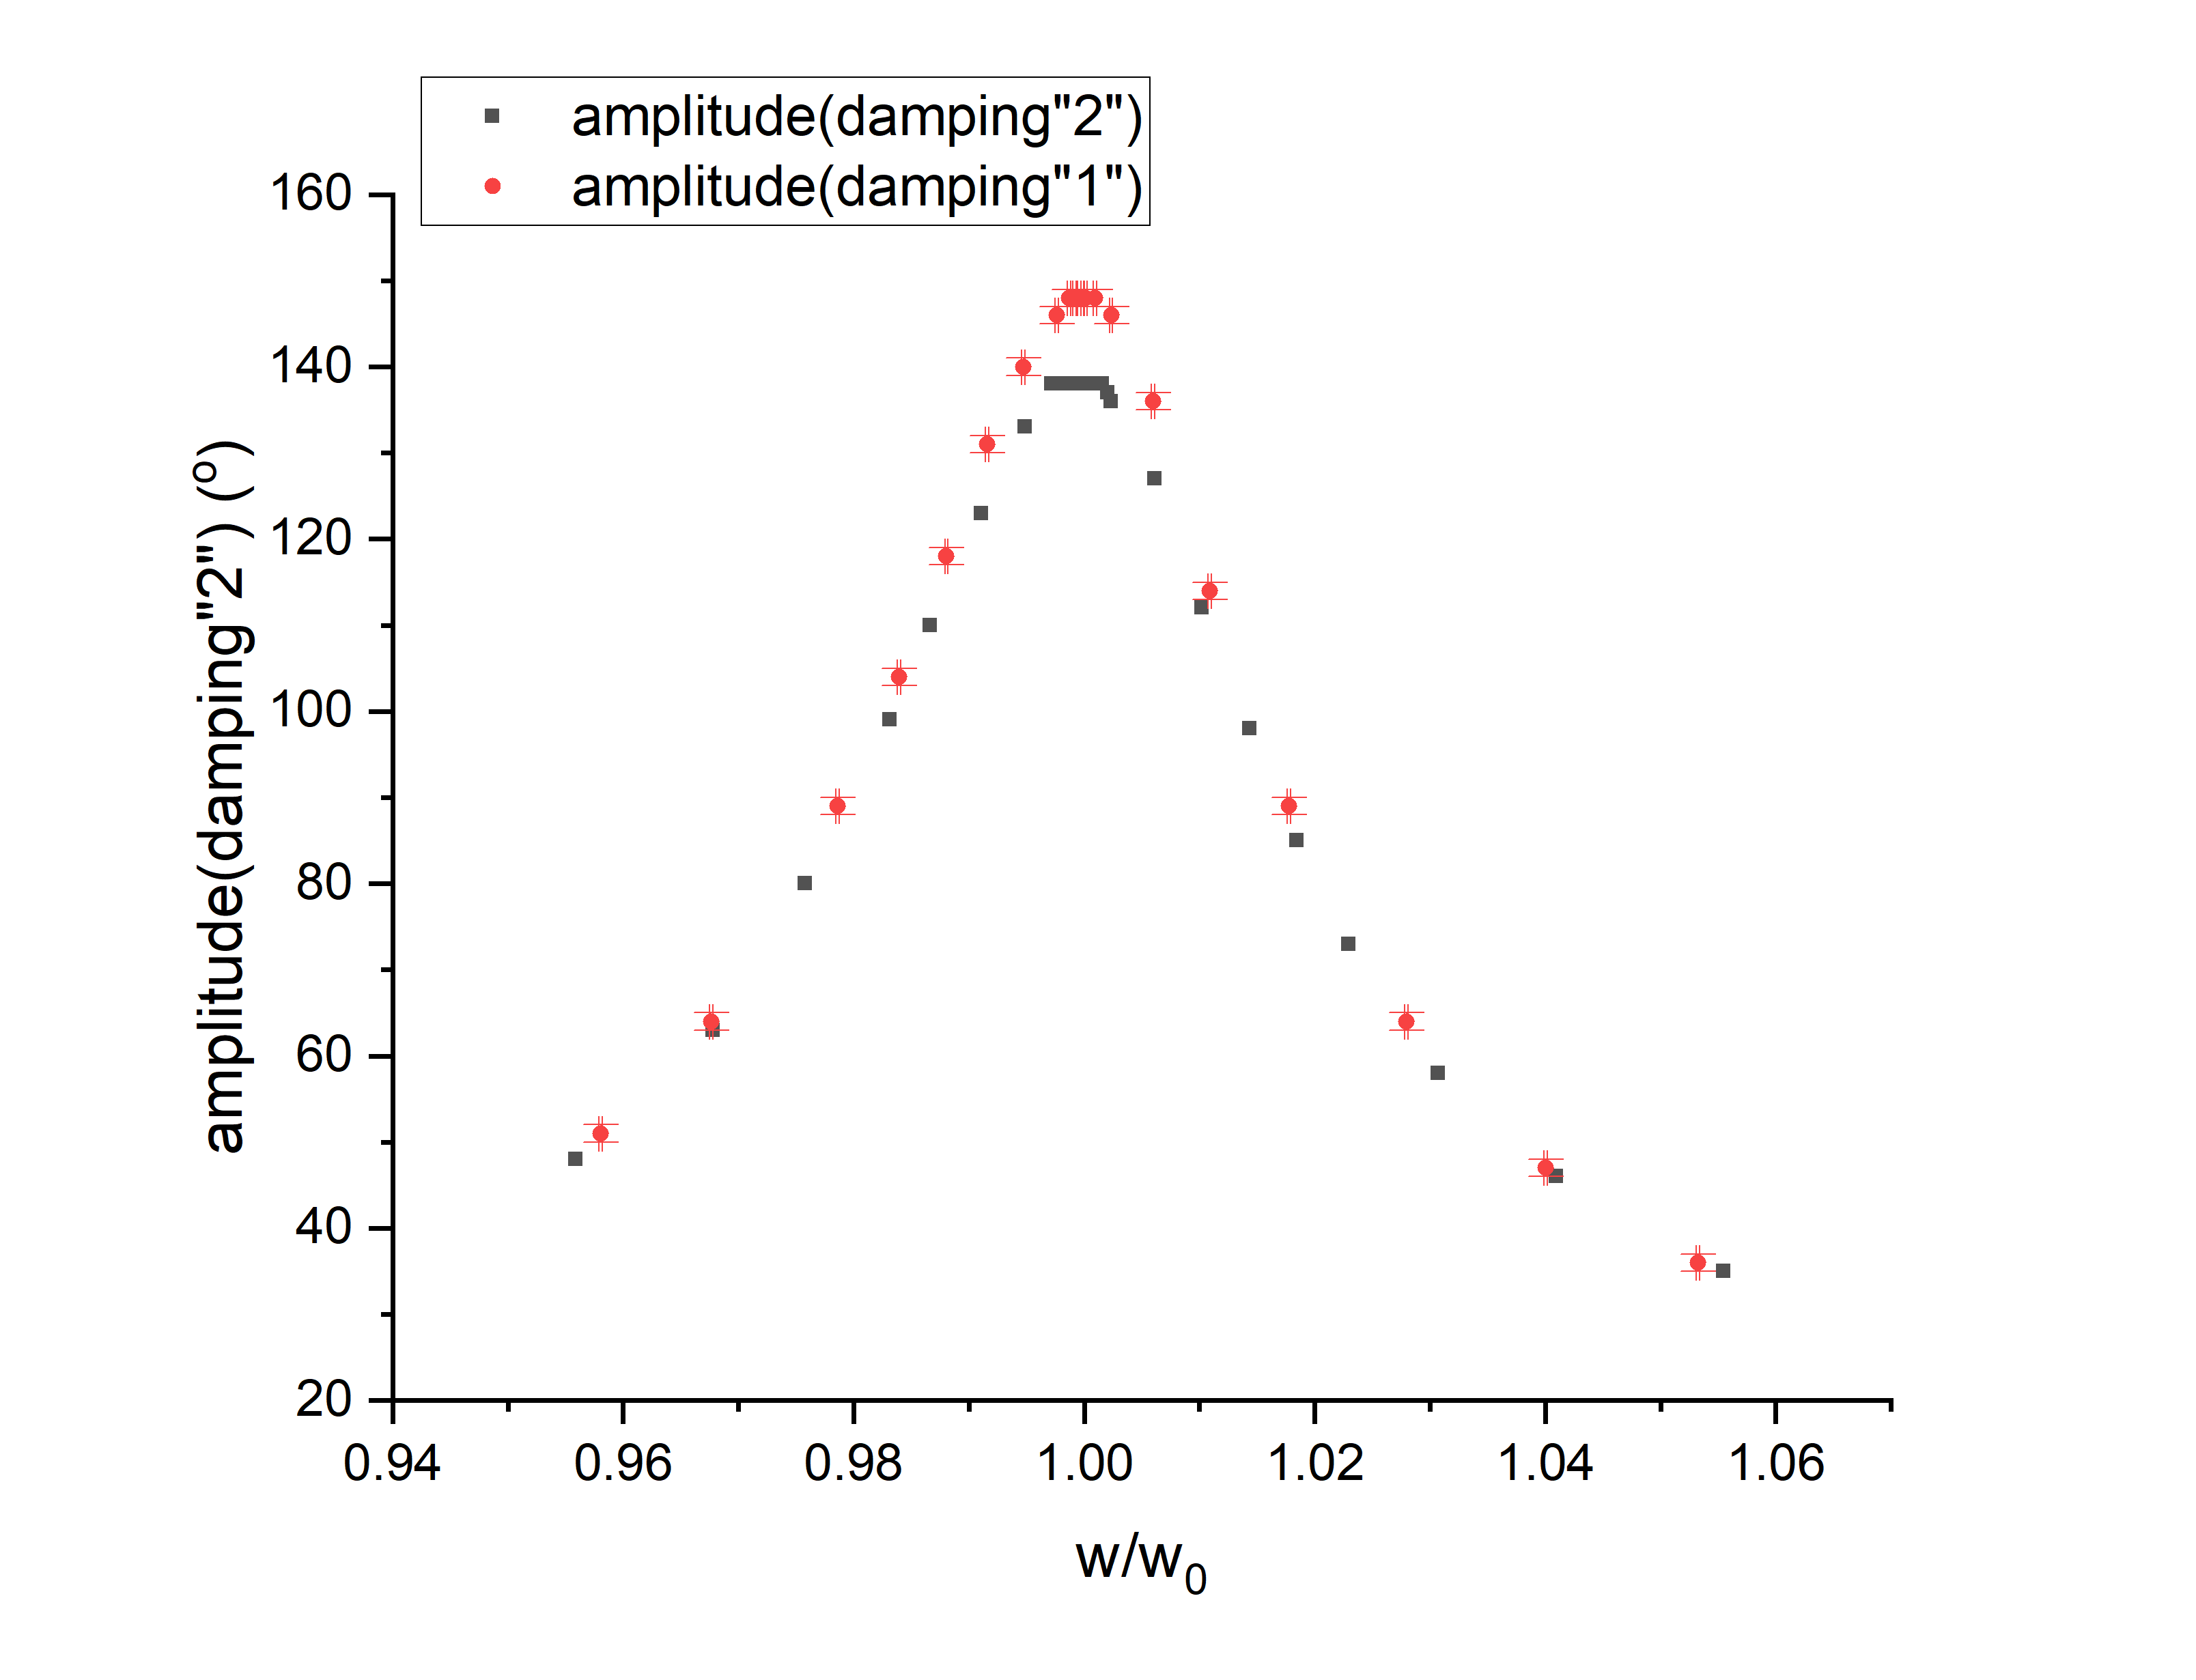
\includegraphics[width=0.8\textwidth]{amplitude.png}
\caption{$\theta_{st}$ vs. $\omega/\omega_0$.}\label{Fig:amplitude}
\end{figure}

\begin{figure}[htbp]
\centering
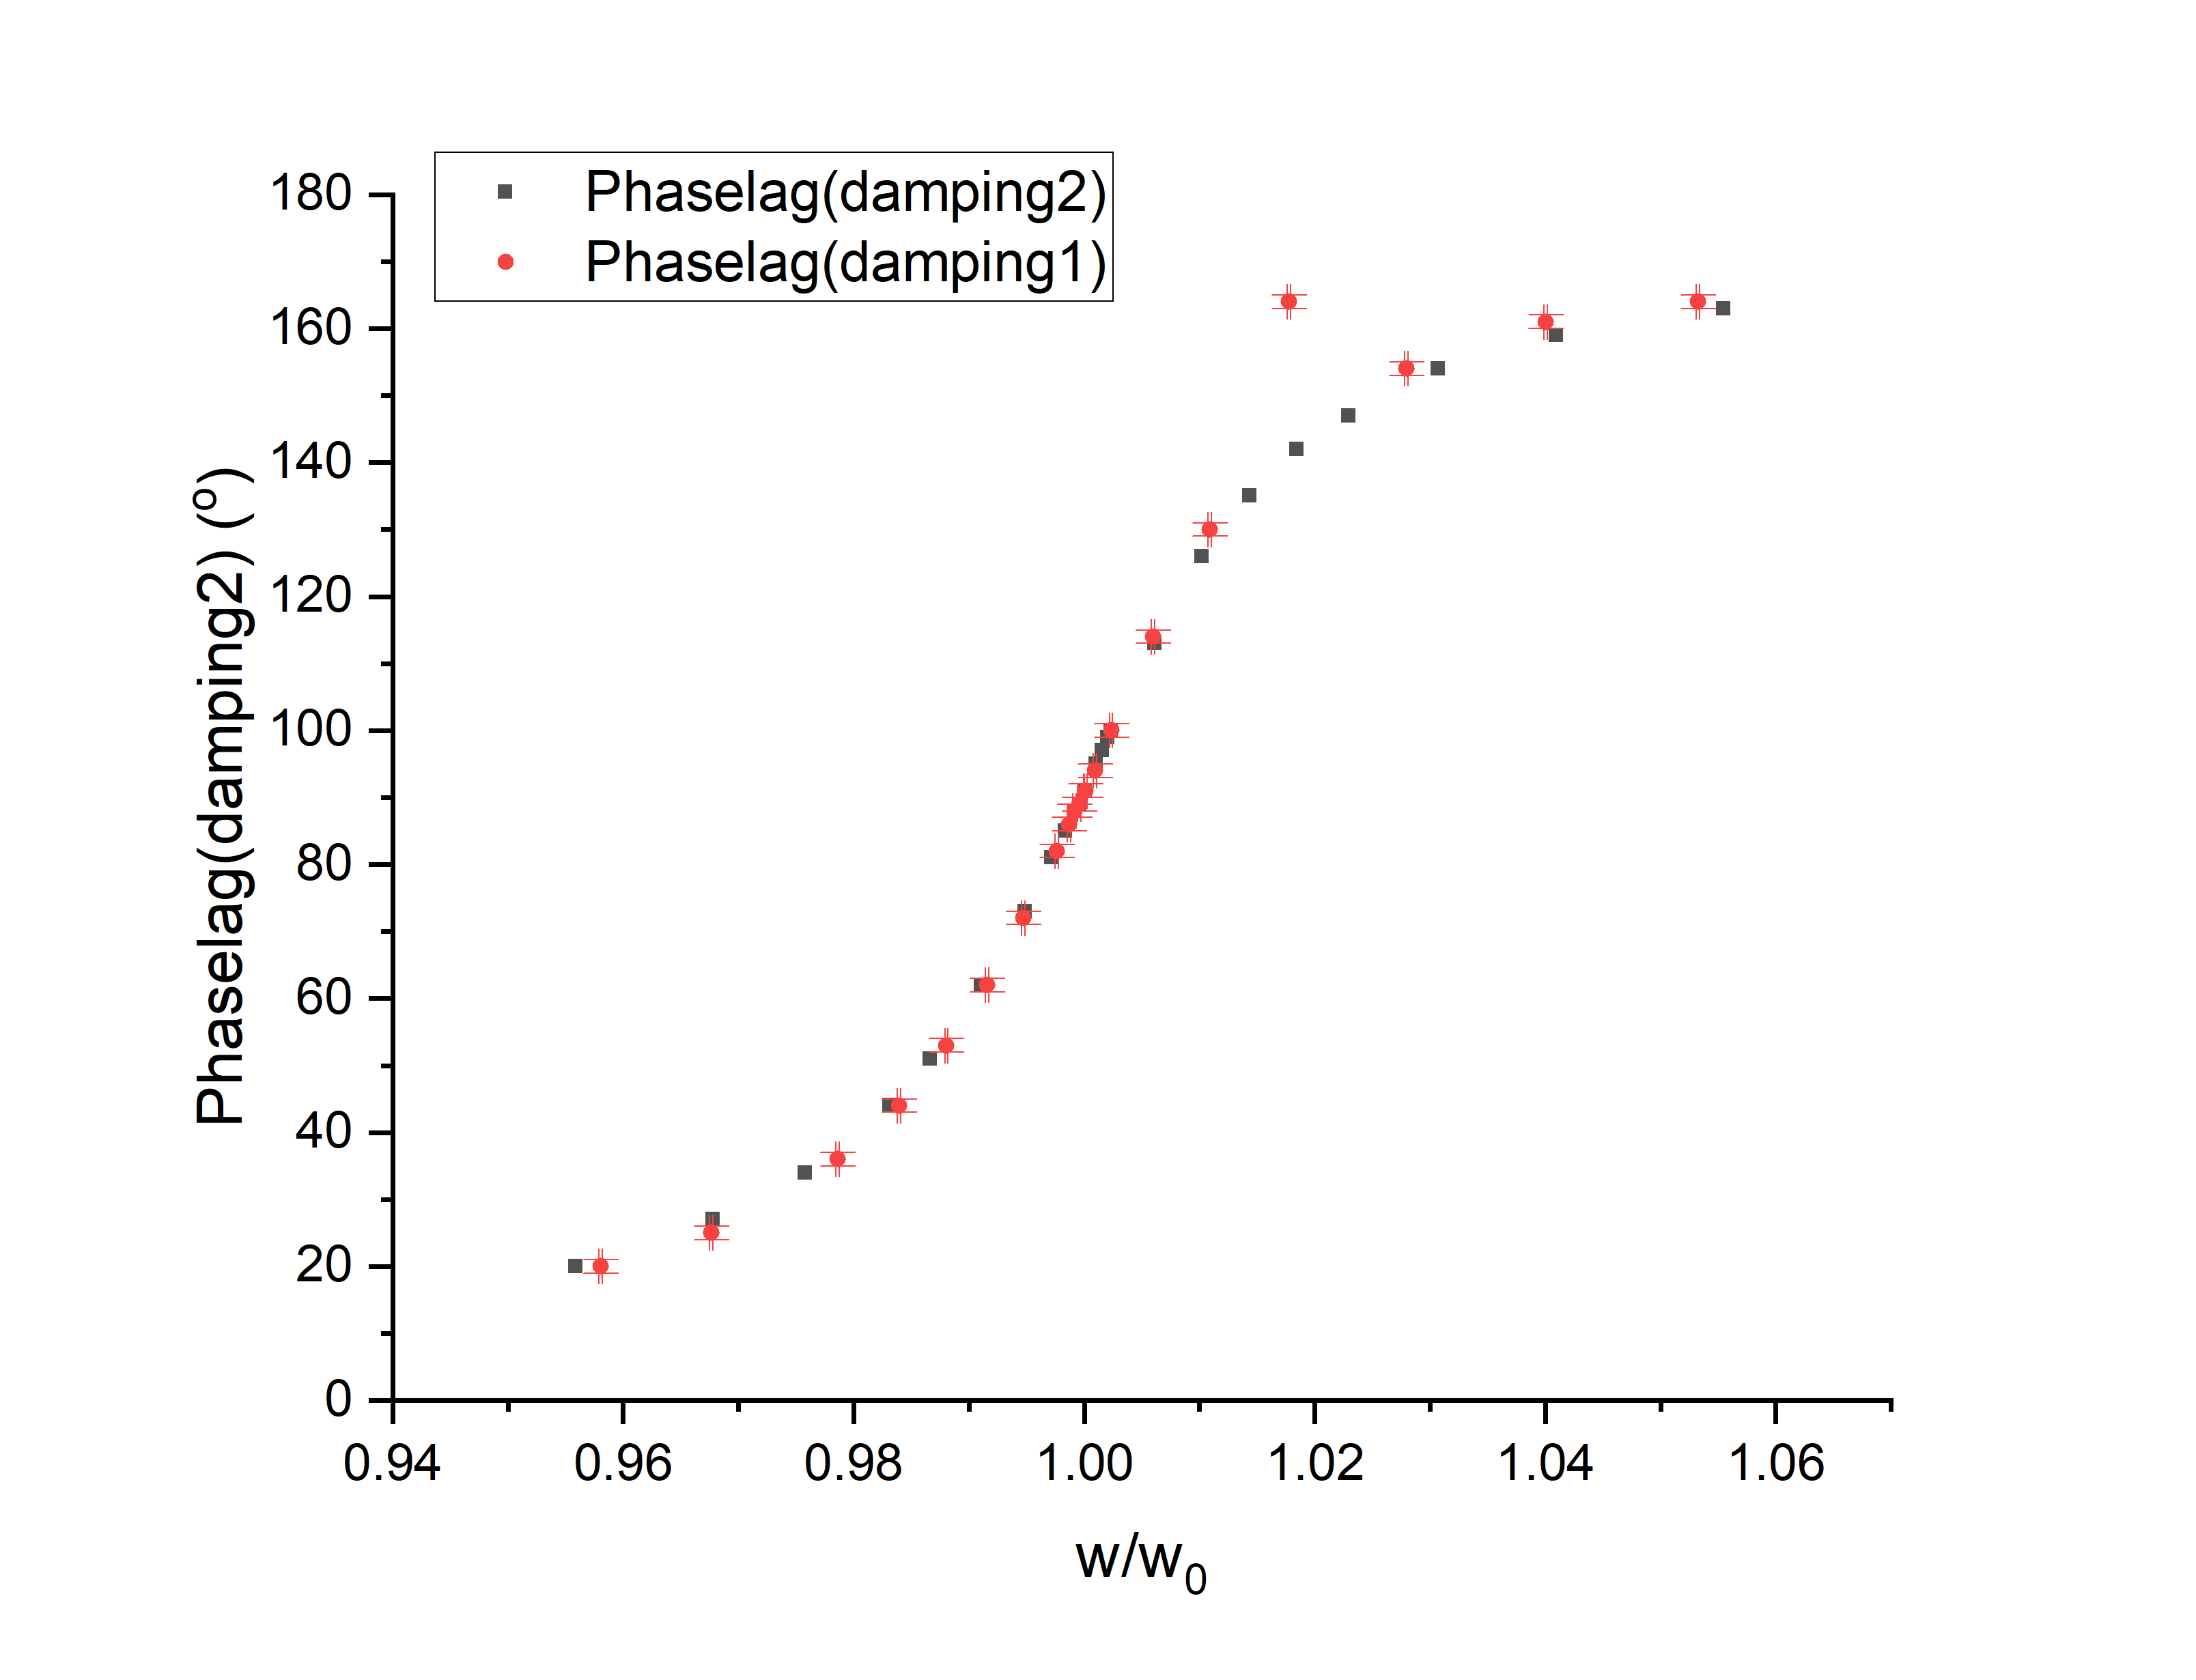
\includegraphics[width=0.8\textwidth]{phaselag.png}
\caption{$\varphi$ vs. $\omega/\omega_0$.}\label{Fig:phaselag}
\end{figure}

\newpage

\section{Conclusions and Discussion}

\subsection{Measurement of natural frequency}

The relative uncertainty of the measurement of this part is 0.01 \%, which suggests that our experiment is of high precision. However, the existing air drag may make the natural frequency of our system a bit 'unnatural' and thus cause error to our measurement.

\subsection{Measurement of damping coefficient}

The relative uncertainty of the measured $\beta$ is 6.16 \%, which is rather high. Some factors may result in the uncertainty and cause error:
\begin{enumerate}
\item The air drag may influence our oscillation system and thus cause error.
\item The low resolution of the device we used is 1$^\circ$, which is relatively large. It may result in the great uncertainty.
\end{enumerate}

\subsection{Measurement of  $\theta$ vs. $\omega$ and $\varphi$ vs. $\omega$ characteristics}
The plotted graphs are shown in Figure \ref{Fig:amplitude} and \ref{Fig:phaselag}. And the corresponding uncertainties are showed in Table \ref{Tab:graphdamping2} and \ref{Tab:graphdamping1}. The shape of the two plottings basically conforms to the theoretical graph as shown in Figure 1. However, note that the fourth circle point from the left in Figure \ref{Fig:phaselag} deviates from the plotting obviously. This is because we perform measurement before the oscillation becomes steady. Also, the amplitude about $\omega/\omega_{0} = 1$ is measured to be the same. This is because the low resolution of our device, which is 1\,$^\circ$. 


\subsection{Suggestions}
Here are some tips for the improvement:
\begin{enumerate}
\item Use the device with higher resolution. Also, the flash is rather harmful to the eyes.
\item Try to reduce the air drag, which may cause error to our experiment.
\end{enumerate}



\section{Reference}

\noindent [1] Qin Tian, et al. editor.``VP141 Exercise 5: Damped and Driven Oscillations. Mechanical Resonance''.

\noindent [2] Young and Freedman. \textit{University Physics with Modern Physics}. Chapter 14.

\newpage



\appendix

\section{Uncertainty Analysis}

Please find in the attached pages.



\section{Data Sheet}

Please find in the attached pages.




\end{document}